%                                                                 aa.dem
% AA vers. 9.1, LaTeX class for Astronomy & Astrophysics
% demonstration file
%                                                       (c) EDP Sciences
%-----------------------------------------------------------------------
%
%\documentclass[referee]{aa} % for a referee version
%\documentclass[onecolumn]{aa} % for a paper on 1 column  
%\documentclass[longauth]{aa} % for the long lists of affiliations 
%\documentclass[letter]{aa} % for the letters 
%\documentclass[bibyear]{aa} % if the references are not structured 
%                              according to the author-year natbib style

%
\documentclass{aa}  

%
\usepackage{graphicx}
%%%%%%%%%%%%%%%%%%%%%%%%%%%%%%%%%%%%%%%%
\usepackage{txfonts}
%%%%%%%%%%%%%%%%%%%%%%%%%%%%%%%%%%%%%%%%
%\usepackage[options]{hyperref}
% To add links in your PDF file, use the package "hyperref"
% with options according to your LaTeX or PDFLaTeX drivers.
%
\begin{document} 


   \title{The periodicity of Betelgeuse explained by surface convection}


    \author{{ Q.~Pilate}\inst{1},{ A.~L{\'o}pez Ariste}\inst{1},{ A.~Lavail}\inst{1},{ Ph. Mathias}\inst{1} }

   \institute{IRAP, Universit\'e de Toulouse, CNRS, CNES, UPS.  14, Av. E. Belin. 31400 Toulouse, France 
             }

   \date{Received ...; accepted ...}

% \abstract{}{}{}{}{} 
% 5 {} token are mandatory
 
  \abstract


   \keywords{
               }

   \maketitle
%
%-------------------------------------------------------------------

\section{Introduction}
Betelgeuse is a red super giant star which has been observed by many astronomers for centuries. This star is known as a semi variable star. In the literature, the variability of the light curve of Betelgeuse is mainly explained by pulsation of the atmosphere. The most common periods found in Betelgeuse are the long secondary period (LSP) which is around $2000$ days and there are few known overtones such as $400$ days or $200$ days. Since the great dimming between the end of 2019 and beginning of 2020, those periods have changed. In this article, we attempt to recover the different periods of Betelgeuse using surface convection. The brightness of Betelgeuse is linked to the giant convective cells present at the surface. Hence, the light curve will be affected by the size and the number of convective cells at the surface. Betelgeuse has been observed almost weekly by the telescope Bernard Lyot at Pic du Midi in France, over a decade. We are also able to produce images of Betelgeuse using linear polarization. Those two points combined allowed us to produce a movie of the surface of Betelgeuse over the last ten years. Using this movie, we try to recover the periodicity of the light curve of Betelgeuse. 

\section{Method}

Trying to find periods in an astrophysical context can be difficult due to the unevenly spaced observed data. To overcome this issue, we use the Lomb-Scargle (LS) periodogram. For a given set of data, it fits a periodic signal using least squares method, for each frequency between the first and the last observation. The better the periodic signal fits the data, the higher the power attributed to the frequency. We used the LS periodogram in the linear polarization and intensity data first. We can see in fig.\ref{LS Intensity} that we recover the LSP around 2000 days. For lower frequencies (i.e periods higher than 2000 days), the signal is attributed to cross correlation. It appears that there is a small signal around $0.003 d^{-1}$ ($\sim 333$ days) but it is hard to affirm that it corresponds a net signal or noise. The LS periodogram of stokes Q shows no LSP but rather shows two periods : one at 0.002 (500 days) and one at 0.005 (200 days). The second one may correspond to an overtone of the fundamental mode that has already been motioned in the literature but the one at 500 days has never been found. From the LS of stokes U, we recover the LSP but there is no clear signal for the other frequencies. Since the LSP is not present in stokes Q but only in stokes I and U, we attribute this frequency to stochastic events. To go further, we examine the LS periodogram of the displacement of the photo-center of Betelgeuse. From the polarimetric data of the TBL, we can produce images of Betelgeuse and follow its photo-center displacement, producing "movies" of Betelgeuse. However, our images are very dependant of the initial parameters to fit the observed profile. To overcome this issue, we computed movies of Betelgeuse 100 times, with a 100 initial different parameters.  Figure \ref{LS narval + neonarval} shows the LS of the data from narval and neo narval up to 2023 for the 100 movies, whereas fig.\ref{LS narval} shows the LS only for narval data. We see that by using only the narval data, we find two peaks in the LS periodogram: one at $\sim 330$ days and another one at $\sim 420$ days. However, those peaks are less clear with neo narval (which was added right after the great dimming of Betelgeuse). 

\section{Convection to explain periodicities}

The disappearance of the periodicity of Betelgeuse after the dimming is consistent with the literature. However, our model only involves surface convection. This means that to explain the periodicity of Betelgeuse, we do not need the presence of pulsation of the atmosphere. Hence, it appears that surface convection is enough to explain the different periods of Betelgeuse. Concerning the stokes profile, we recover the LSP from stochastic effects. The linear polarization of Betelgeuse is also attributed to convective cells. Thus, our images of Betelgeuse and linear polarization can recover the periodicity of Betelgeuse by only involving surface dynamics which are linked to convection. To support the argument that the variability of Betelgeuse is due to the convection, we can also look at the timescale of convective structures. The surface of RSGs are made of giant convective cells, that live from months to years. Once again, the periodicity of $400$ days, or even the LSP of 2000 days often found in RSGs, are probably linked to the timescale where those super granules evolve. The LS of stokes Q shows a strong signal around 500 days around $\sim 50$ km/s. This signal can be explained by convective plumes that are beyond the limb. Those event happen occasionally in Betelgeuse, but might explain a periodicity. If a plume rises beyond the limb of Betelgeuse, more light is coming toward us, leading to an increase in luminosity. After a few month, the plume falls back and the luminosity of Betelgeuse decreases. Another explanation might be due to choc waves.


\begin{figure}
    \centering
    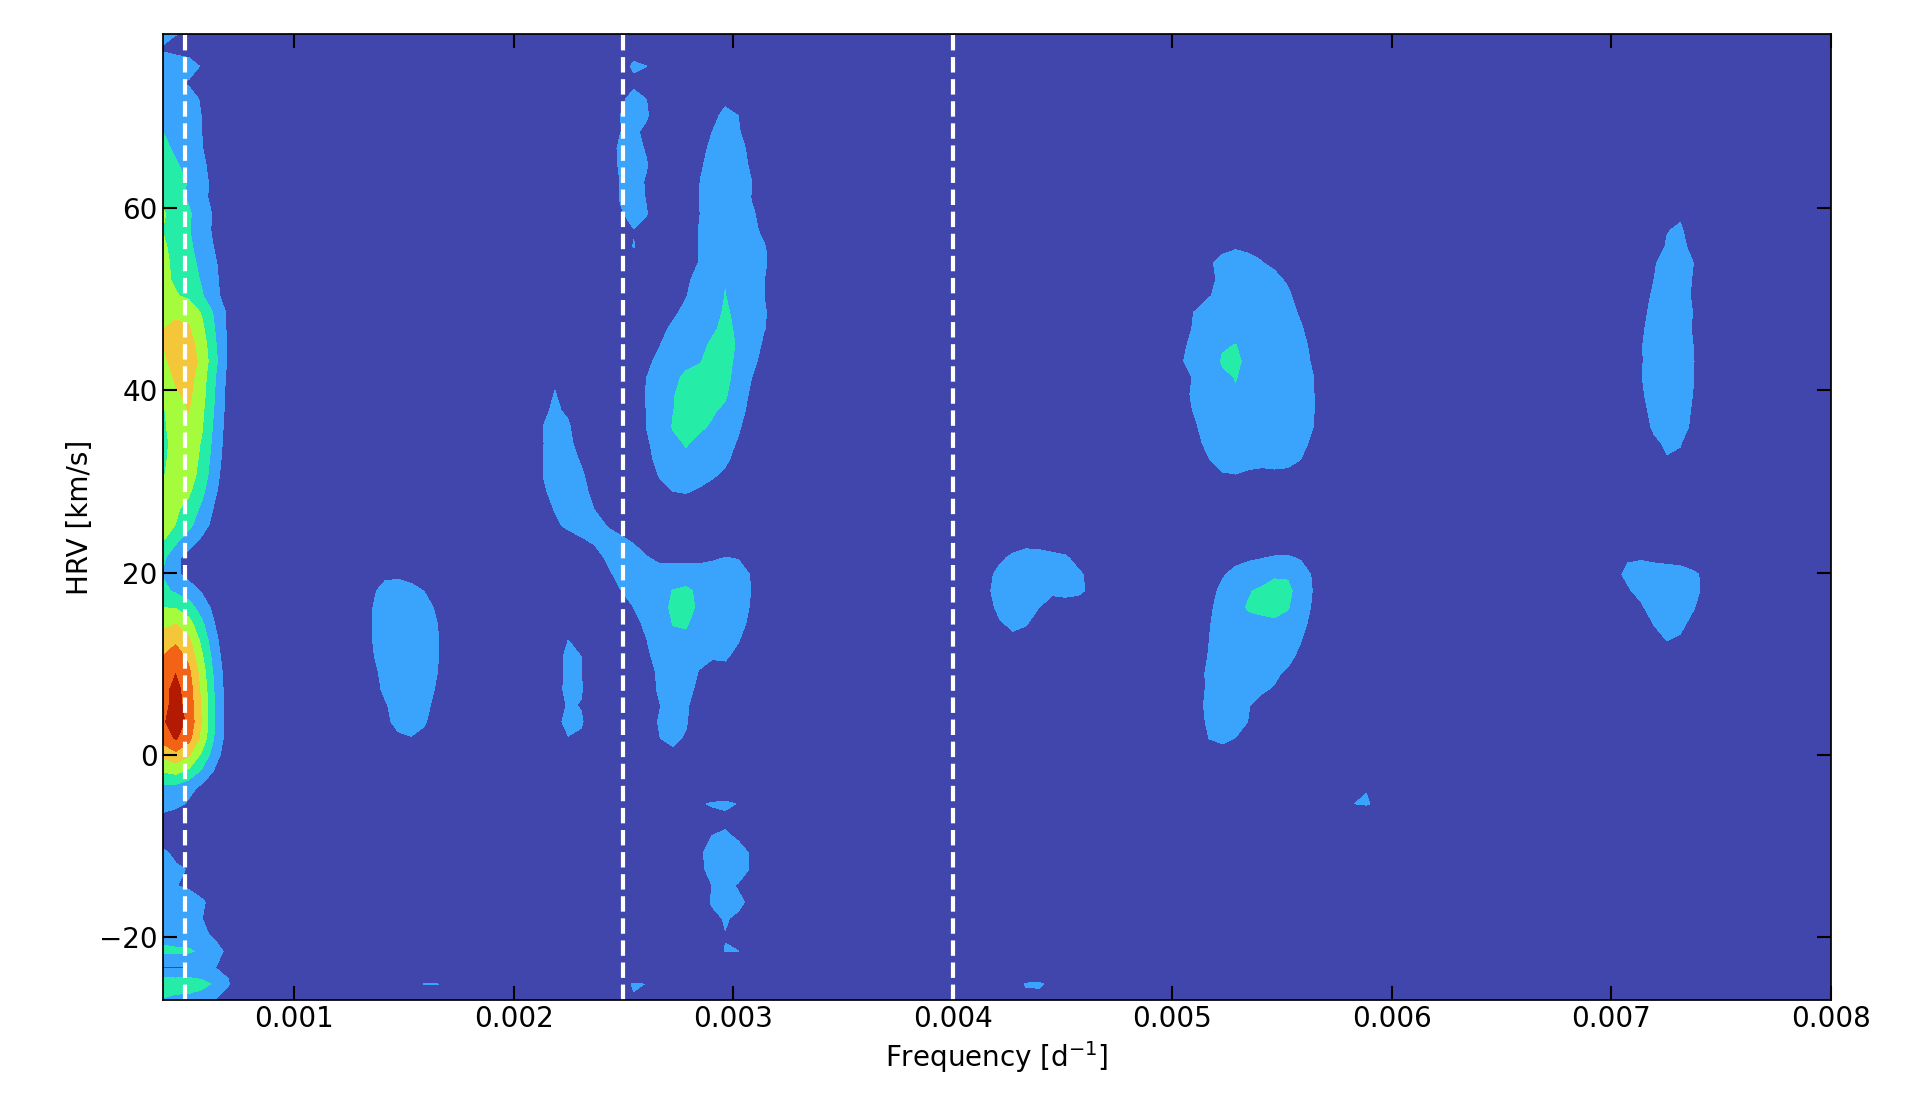
\includegraphics[width=0.4\textwidth]{LS Intensity.png}
    \caption{stokes I}
    \label{LS Intensity}
\end{figure}
\begin{figure}
    \centering
    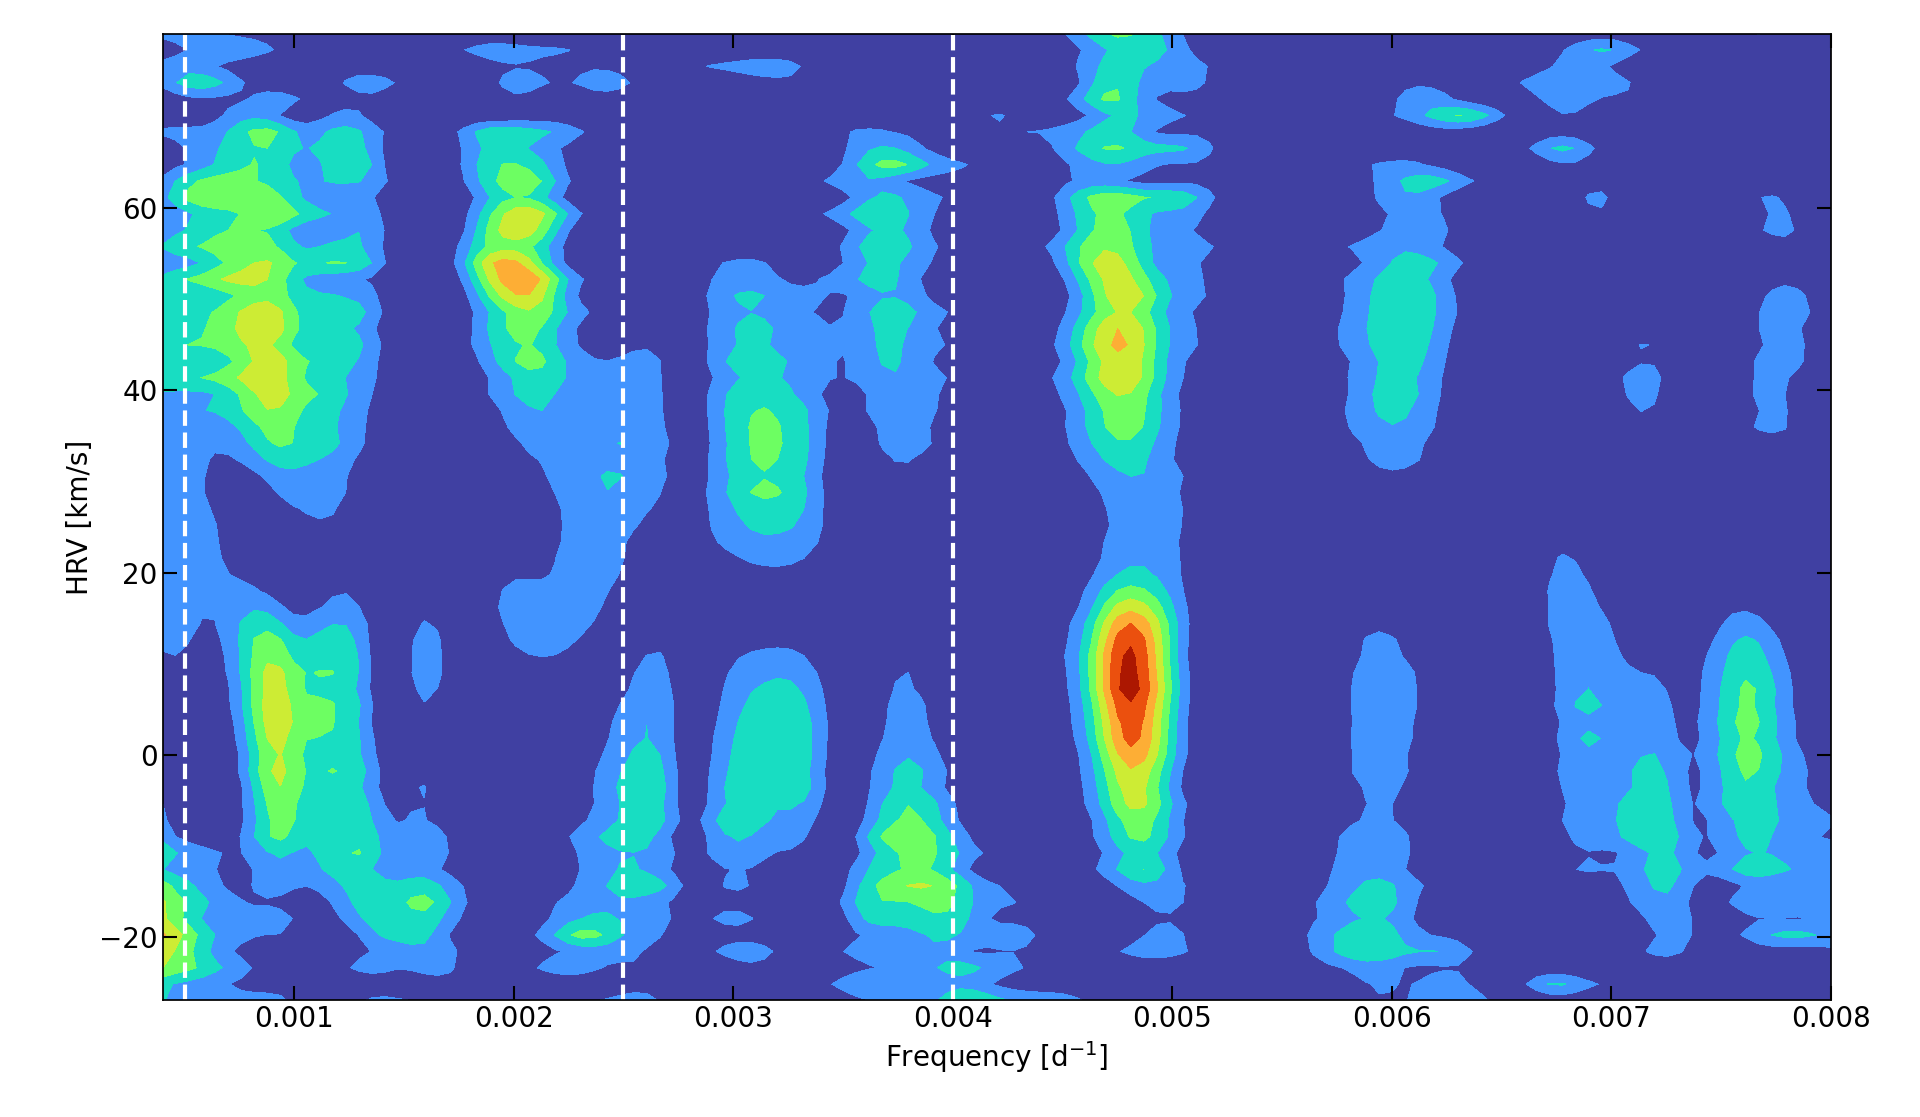
\includegraphics[width=0.4\textwidth]{LS stokes Q.png}
    \caption{stokes Q}
    \label{LS Q}
\end{figure}

\begin{figure}
    \centering
    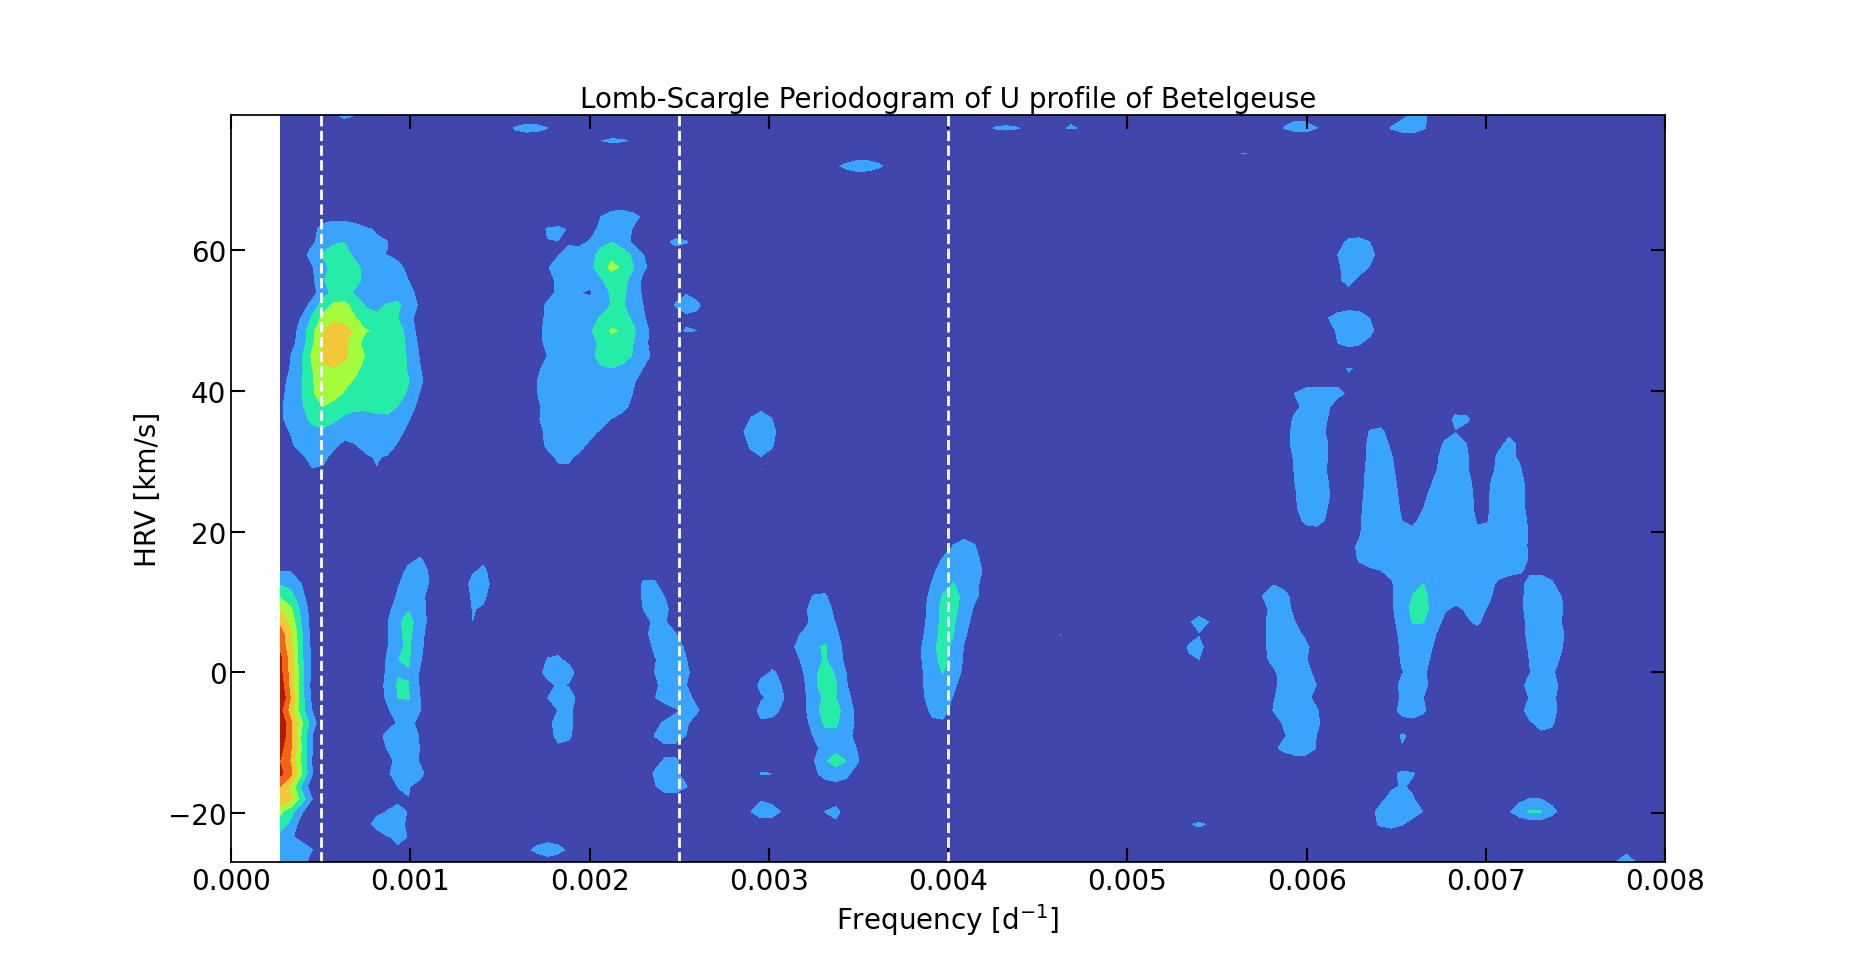
\includegraphics[width=0.4\textwidth]{LS stokes U.png}
    \caption{stokes U}
    \label{LS U}
\end{figure}

\begin{figure}
    \centering
    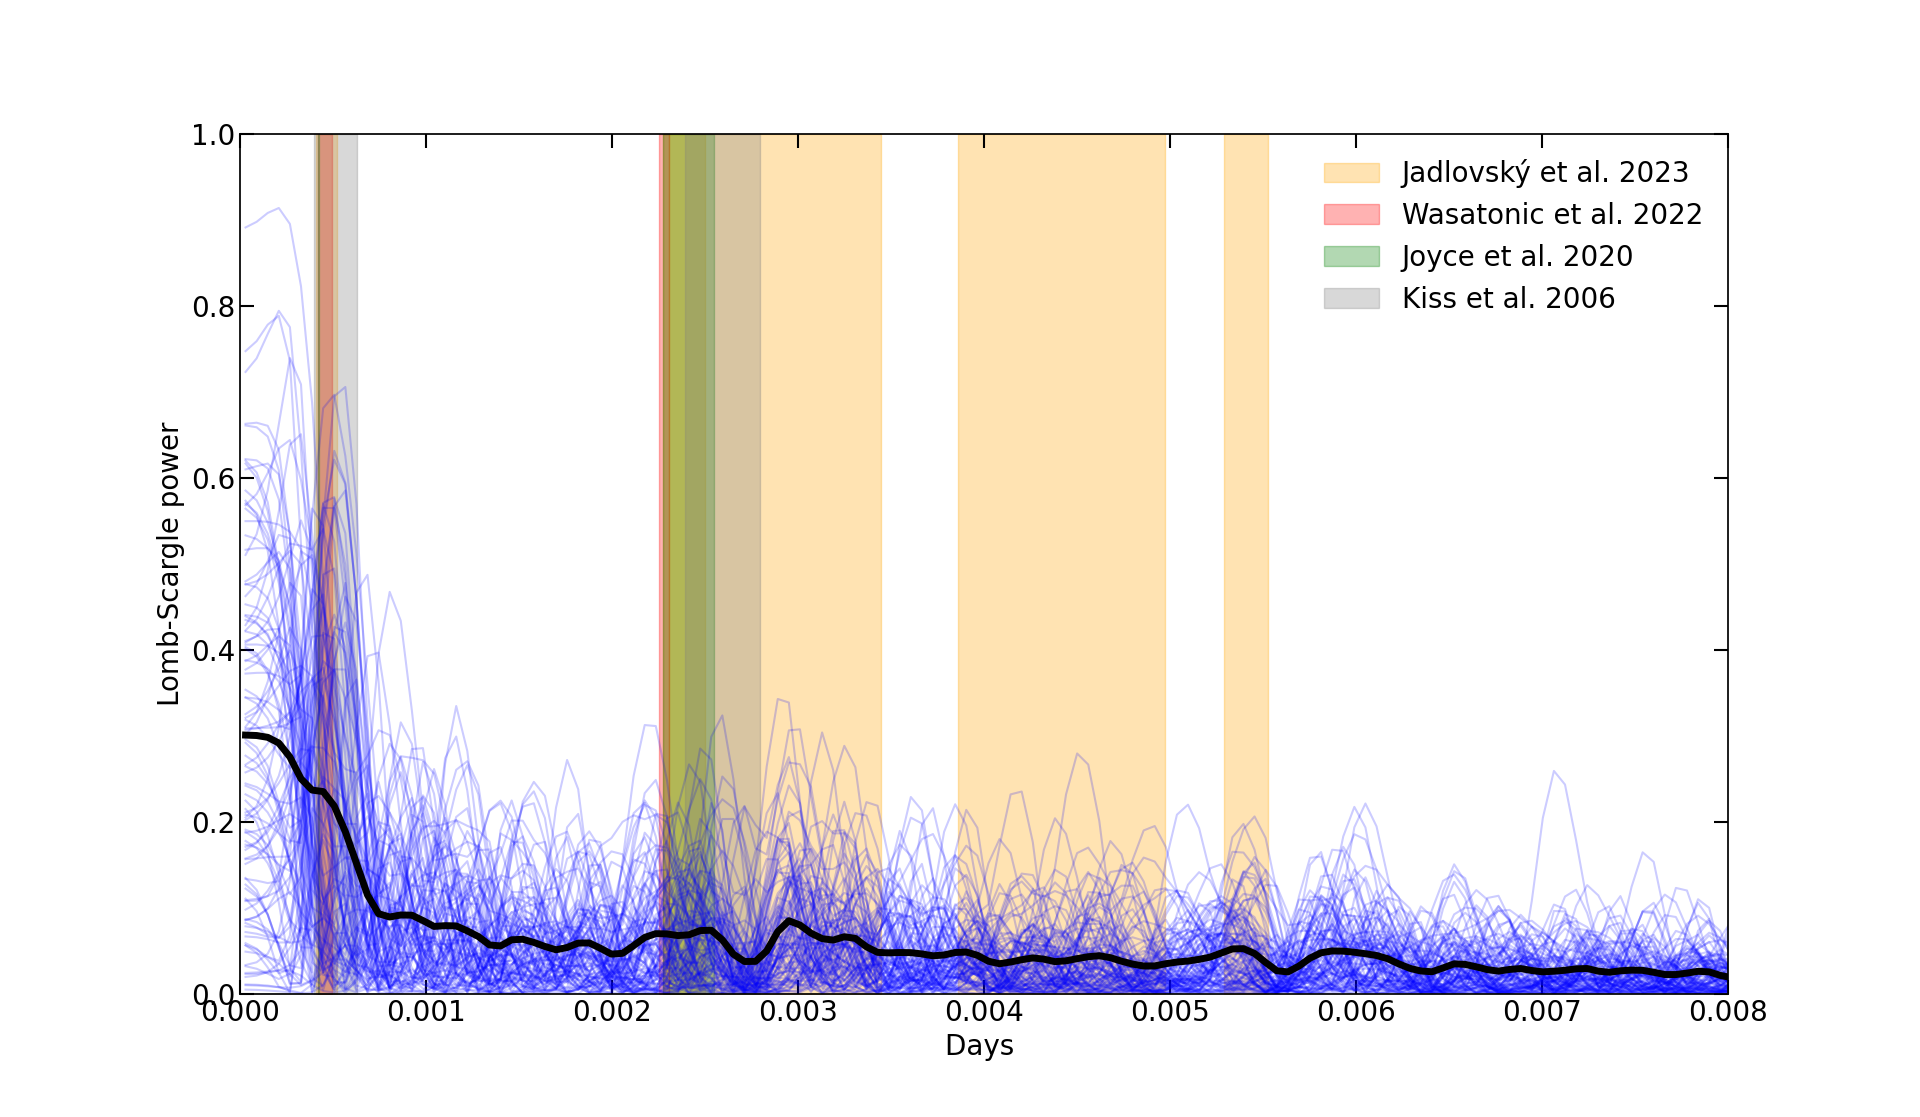
\includegraphics[width=0.4\textwidth]{LS photocentre Narval and Neo Narval.png}
    \caption{narval + neonarval}
    \label{LS narval + neonarval}
\end{figure}

\begin{figure}
    \centering
    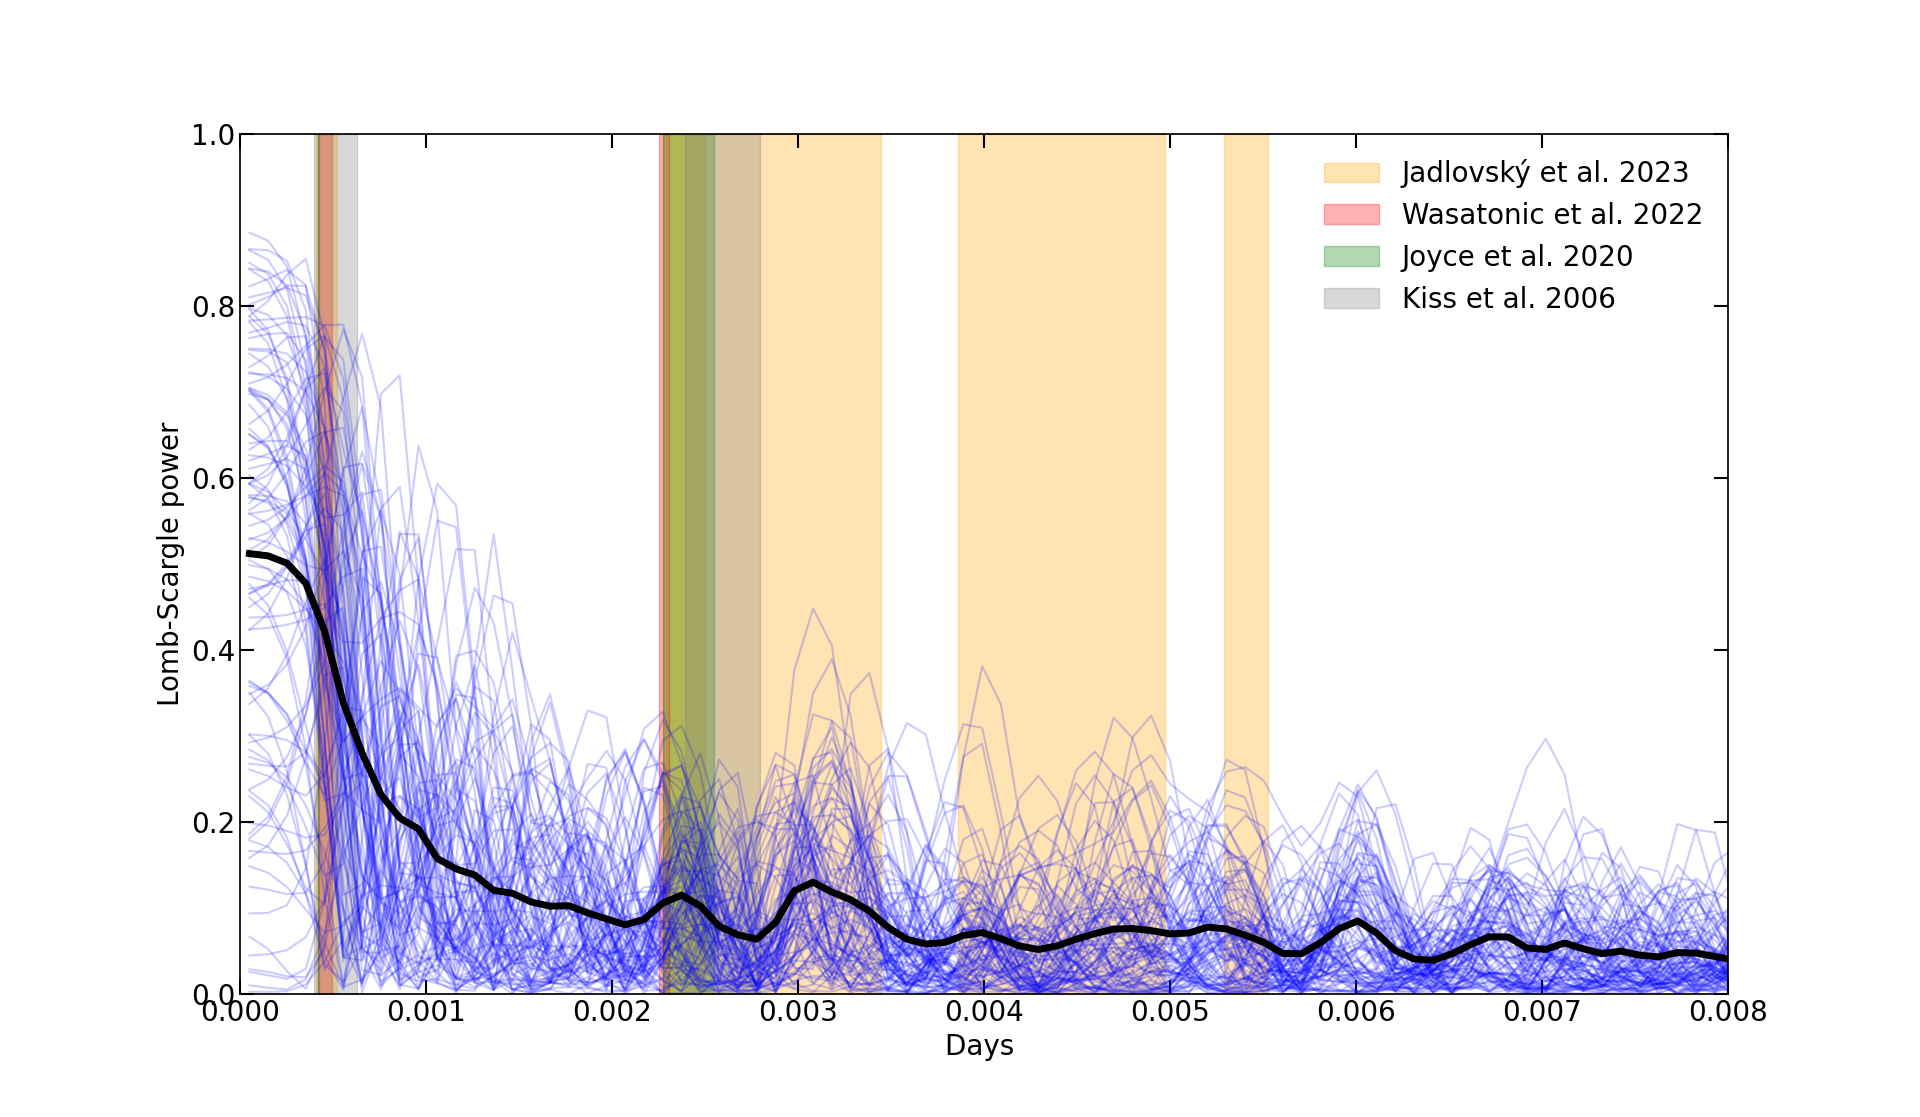
\includegraphics[width=0.4\textwidth]{LS photocentre Narval.png}
    \caption{narval}
    \label{LS narval}
\end{figure}

\end{document}


